\begin{appendices}
%\appendixpage
\noappendicestocpagenum
\addappheadtotoc


\renewcommand{\myfullcite}[1]{\printpublication{#1}.}


% Numbered tab on each paper introduction page.
\newcommand{\papernumbertab}[1]{%
\placetextbox{0.95}{0.75}{%
  \begingroup
  \setlength{\fboxsep}{0pt}%
  \colorbox{black}{\parbox[c][18mm][c]{16.5mm}{\centering\color{white}\Huge\bfseries #1}}%
  \endgroup
}
}

\renewcommand{\appendixname}{Paper}
\chapter{Graph Representation Learning for Software Architecture Recovery}\label{app:publ-arl_2026}
\papernumbertab{I}
\myfullcite{arl_2026}

\vspace{10pt}
\noindent
% TODO: confirm reuse-rights text for ESANN/i6doc.com proceedings before
% printing a notice. Acceptance itself is confirmed (ESANN 2026
% proceedings, ISBN 9782875870964), so the PDF is now included below;
% only the license/reuse sentence is still pending.
% {\footnotesize [reuse-rights notice -- pending confirmation]}
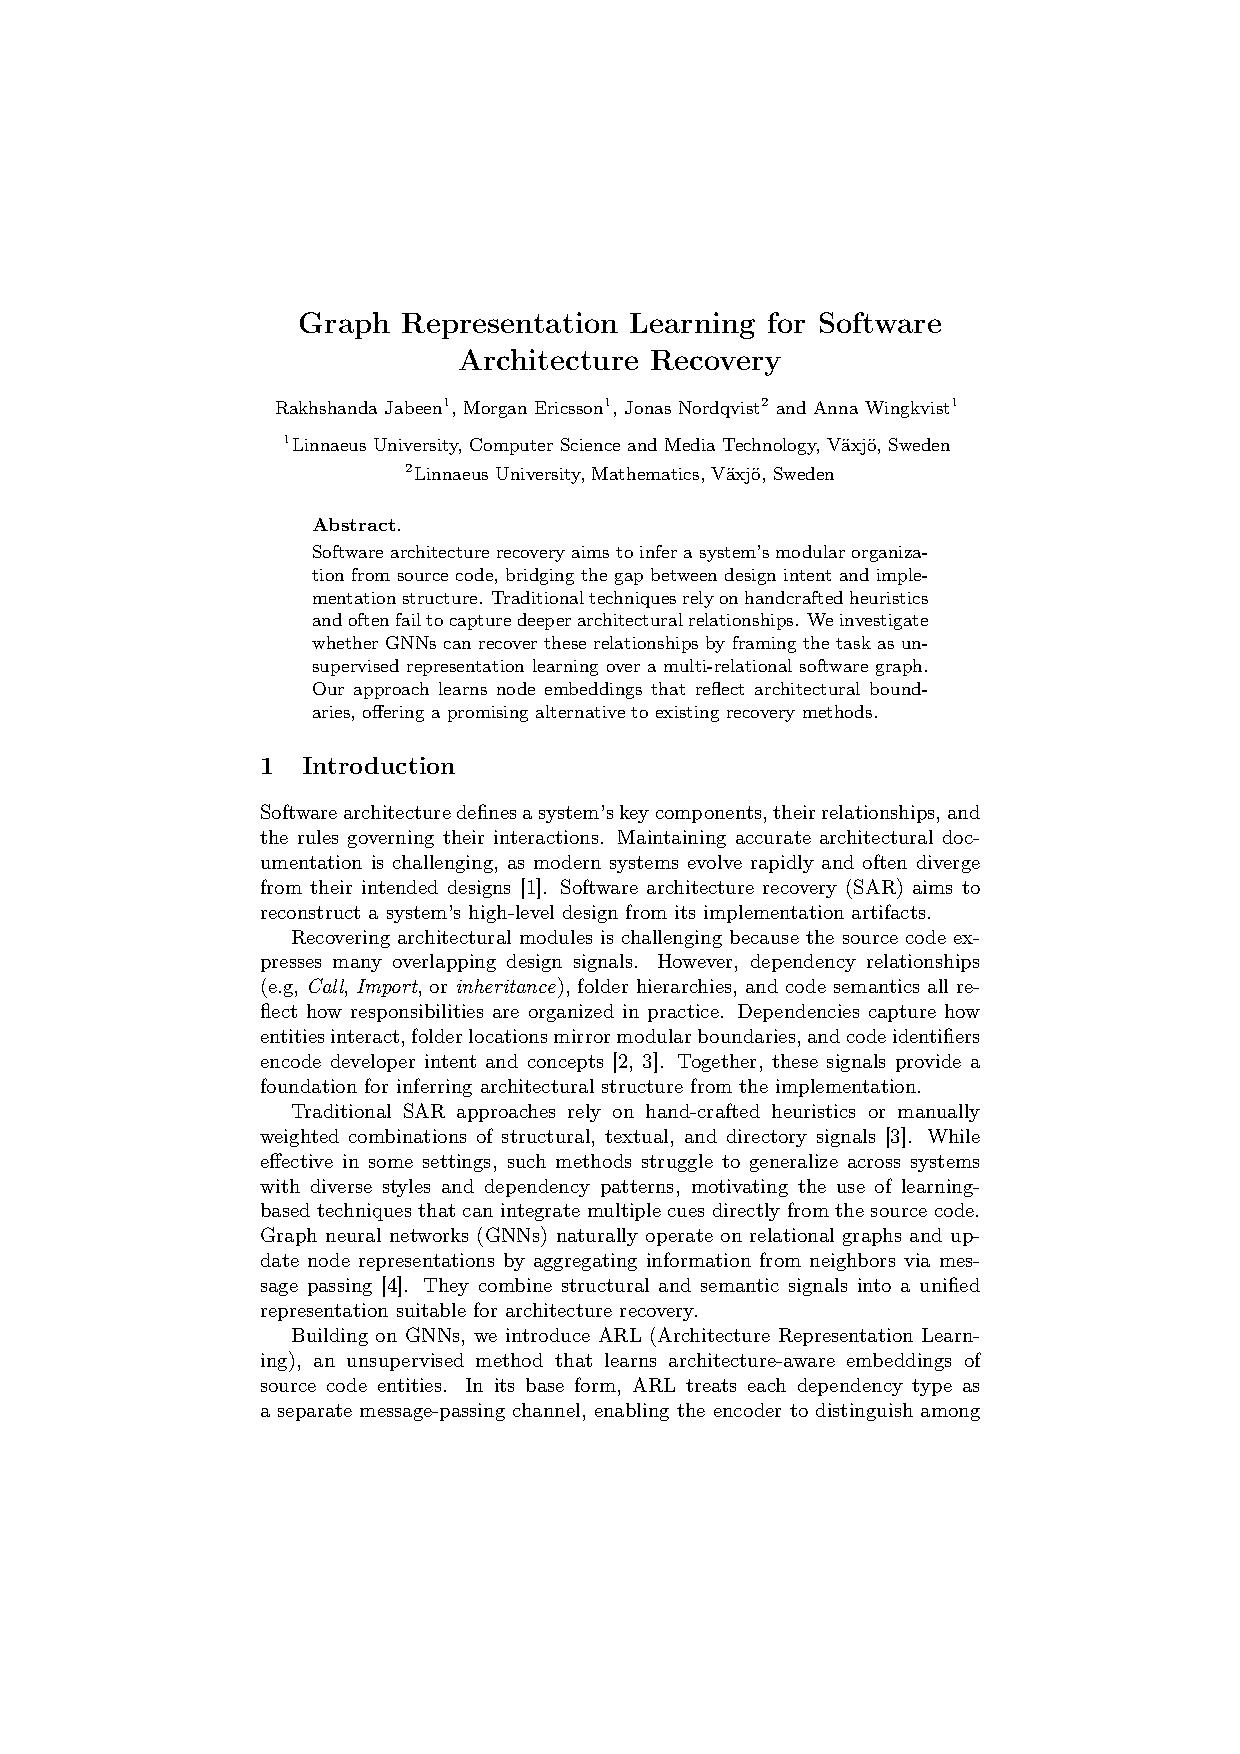
\includepdf[pages=-,pagecommand={}]{papers/ARL.pdf}
% TODO: same as below -- addtotoc deferred until page numbers are known
% from a compiled draft.


\renewcommand{\appendixname}{Article}
\chapter{GAER: Graph Auto-Encoders for Unsupervised Software Architecture Recovery}\label{app:publ-gaer}
\papernumbertab{II}
\myfullcite{gaer}

\vspace{10pt}
\noindent
% TODO: confirm reuse-rights text. PACM Softw. Eng. (FSE) is published by
% ACM -- check whether this appeared under ACM's standard copyright
% transfer (then: "Reprinted under the ACM reuse author rights.", as
% Hoenel used) or under ACM Open / Gold OA (then a CC BY notice with the
% specific license version applies instead). ACM DL blocked automated
% verification for doi 10.1145/3808187 -- confirm manually from the
% copyright-transfer email or the DL page's rights panel.
% {\footnotesize [reuse-rights notice -- pending confirmation]}
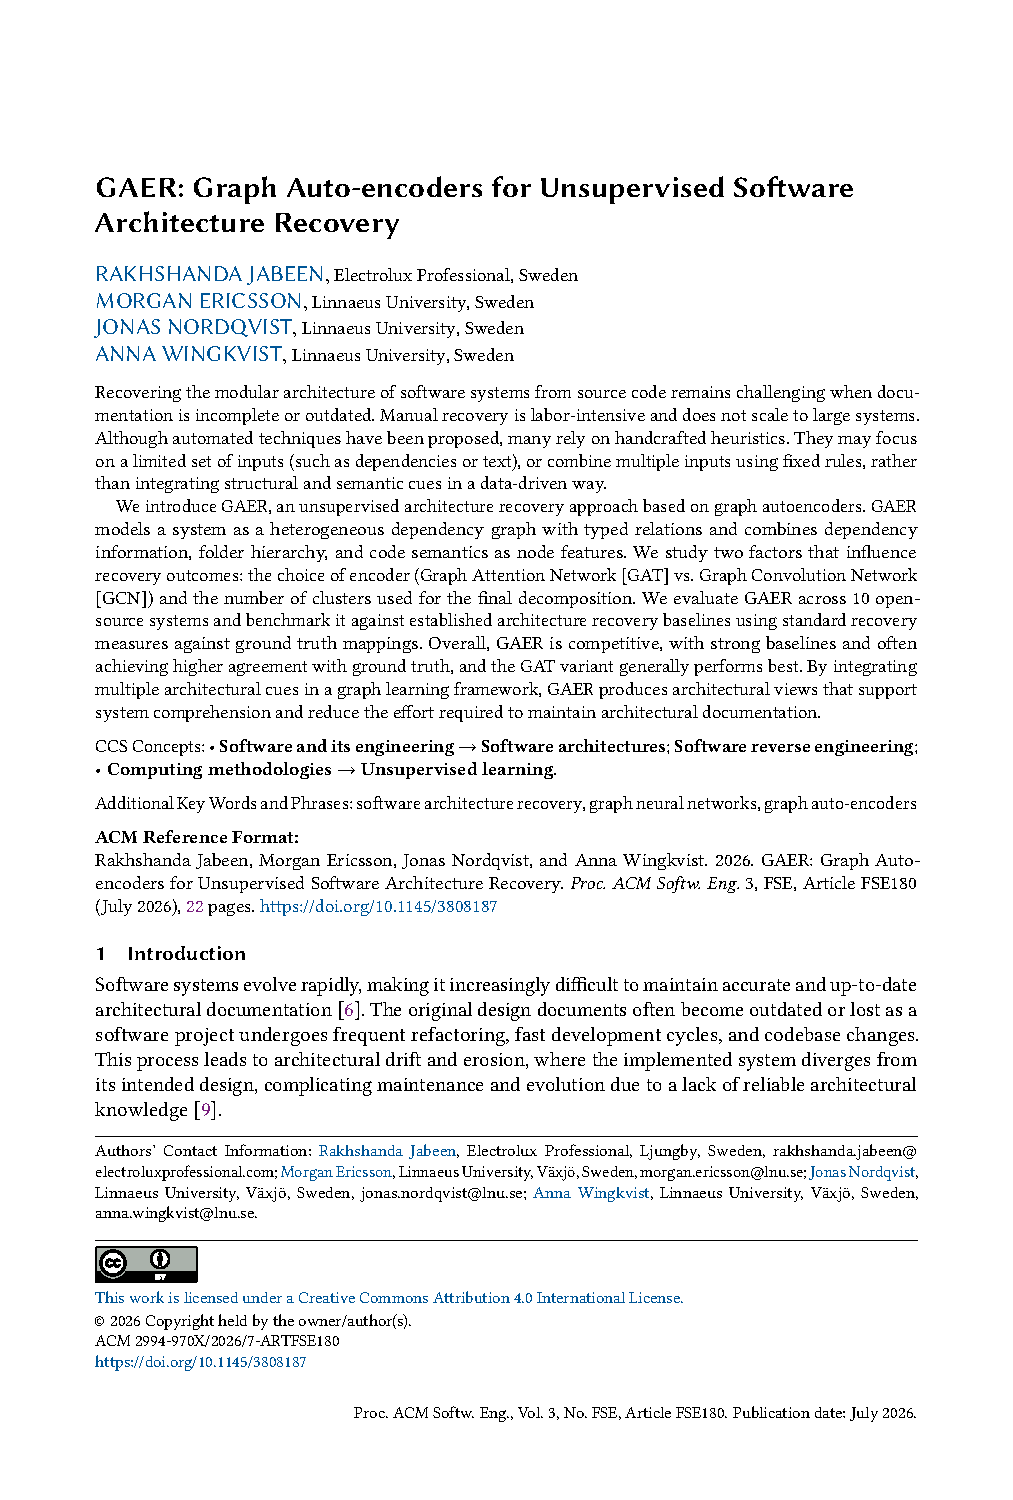
\includepdf[pages=-,pagecommand={}]{papers/GAER.pdf}
% TODO: addtotoc deferred until page numbers are known from a compiled
% draft.


\renewcommand{\appendixname}{Paper}
\chapter{Automatic Code-to-Architecture Mapping with Graph Neural Networks}\label{app:publ-c2a_mapping}
\papernumbertab{III}
\myfullciteur{c2a_mapping}
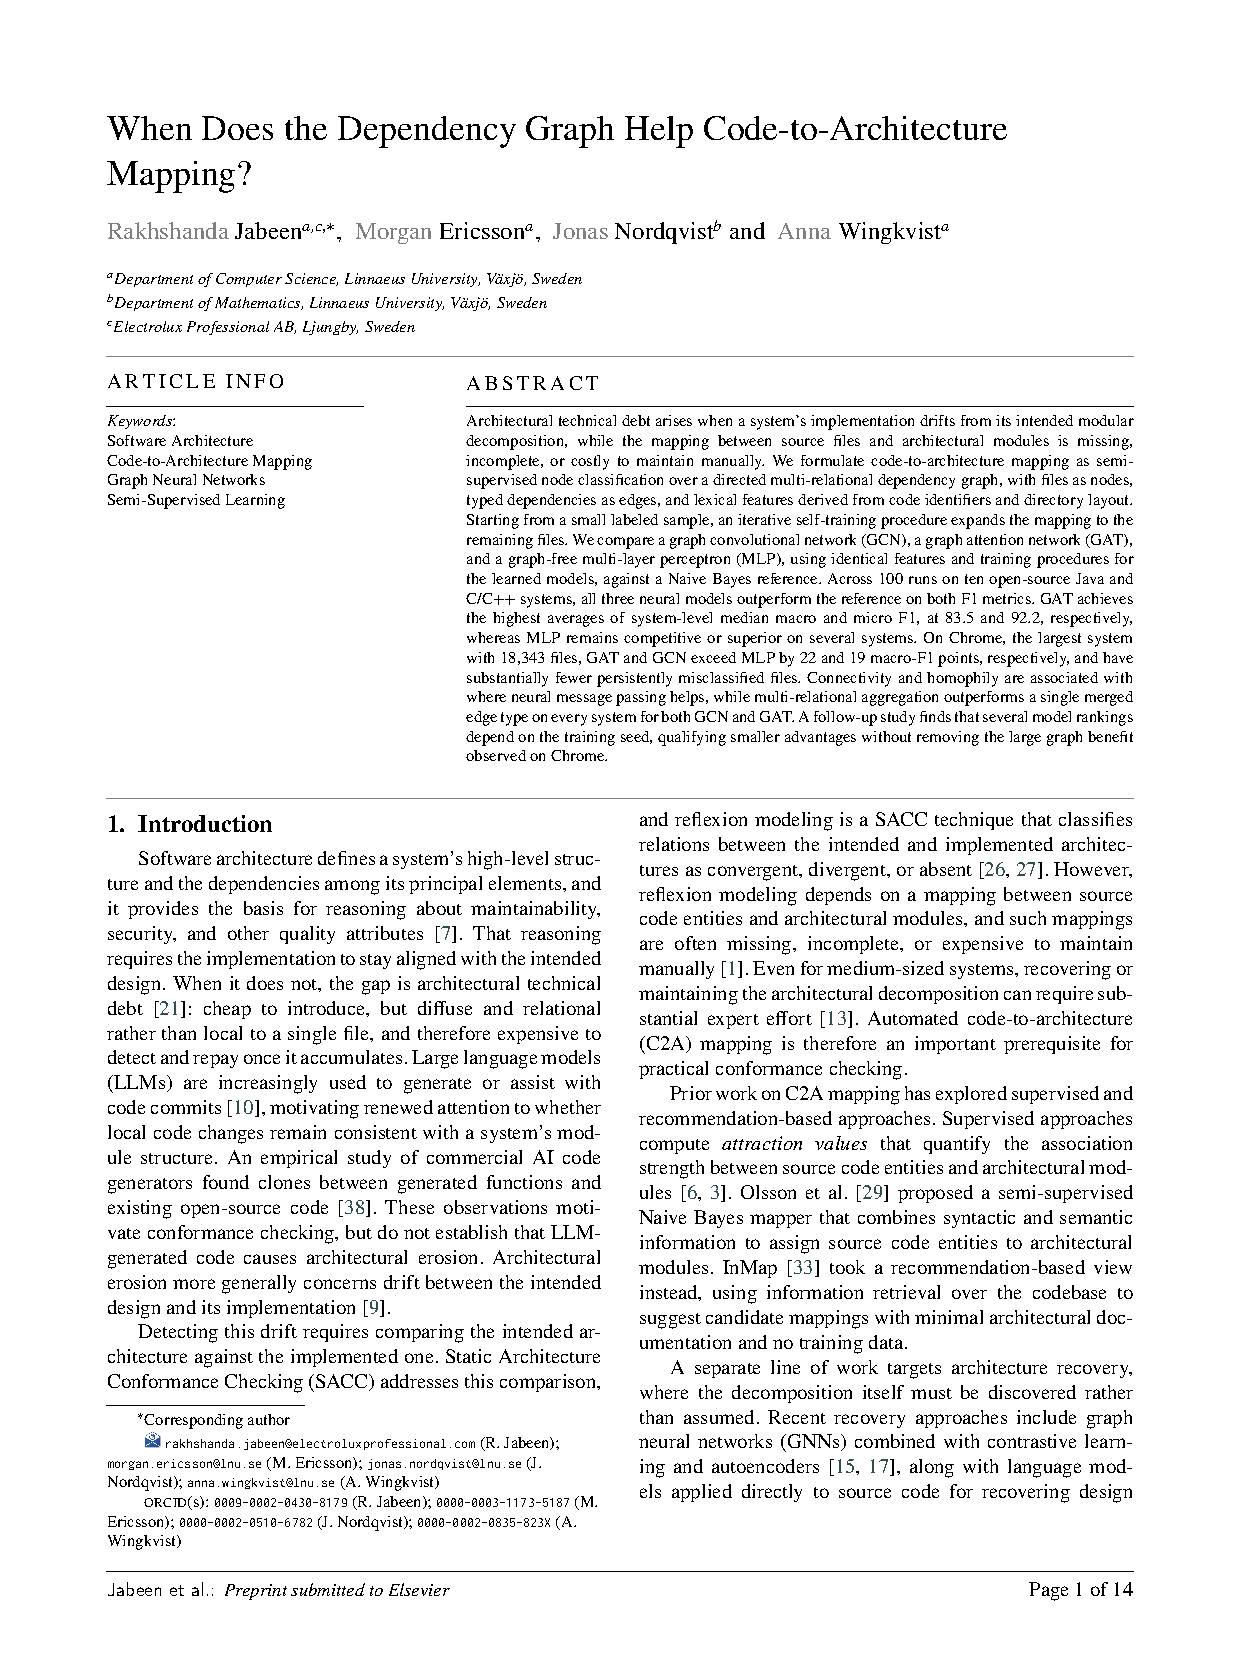
\includepdf[pages=-,pagecommand={}]{papers/C2A_mapping.pdf}
% Manuscript under review -- not yet published, so no reuse-rights
% notice or \includepdf applies. Rendered as a citation marked
% "Under review" until the paper is accepted and a camera-ready PDF exists.



\renewcommand{\appendixname}{Article}
\chapter{Graph Embeddings for Software Architecture Recovery}\label{app:publ-structsar}
\papernumbertab{IV}
\myfullcite{structsar}

\vspace{10pt}
\noindent
{\footnotesize Reprinted under the Creative Commons Attribution 4.0 International License (CC~BY~4.0). Copyright \copyright{} 2026 Nordic Machine Intelligence.}
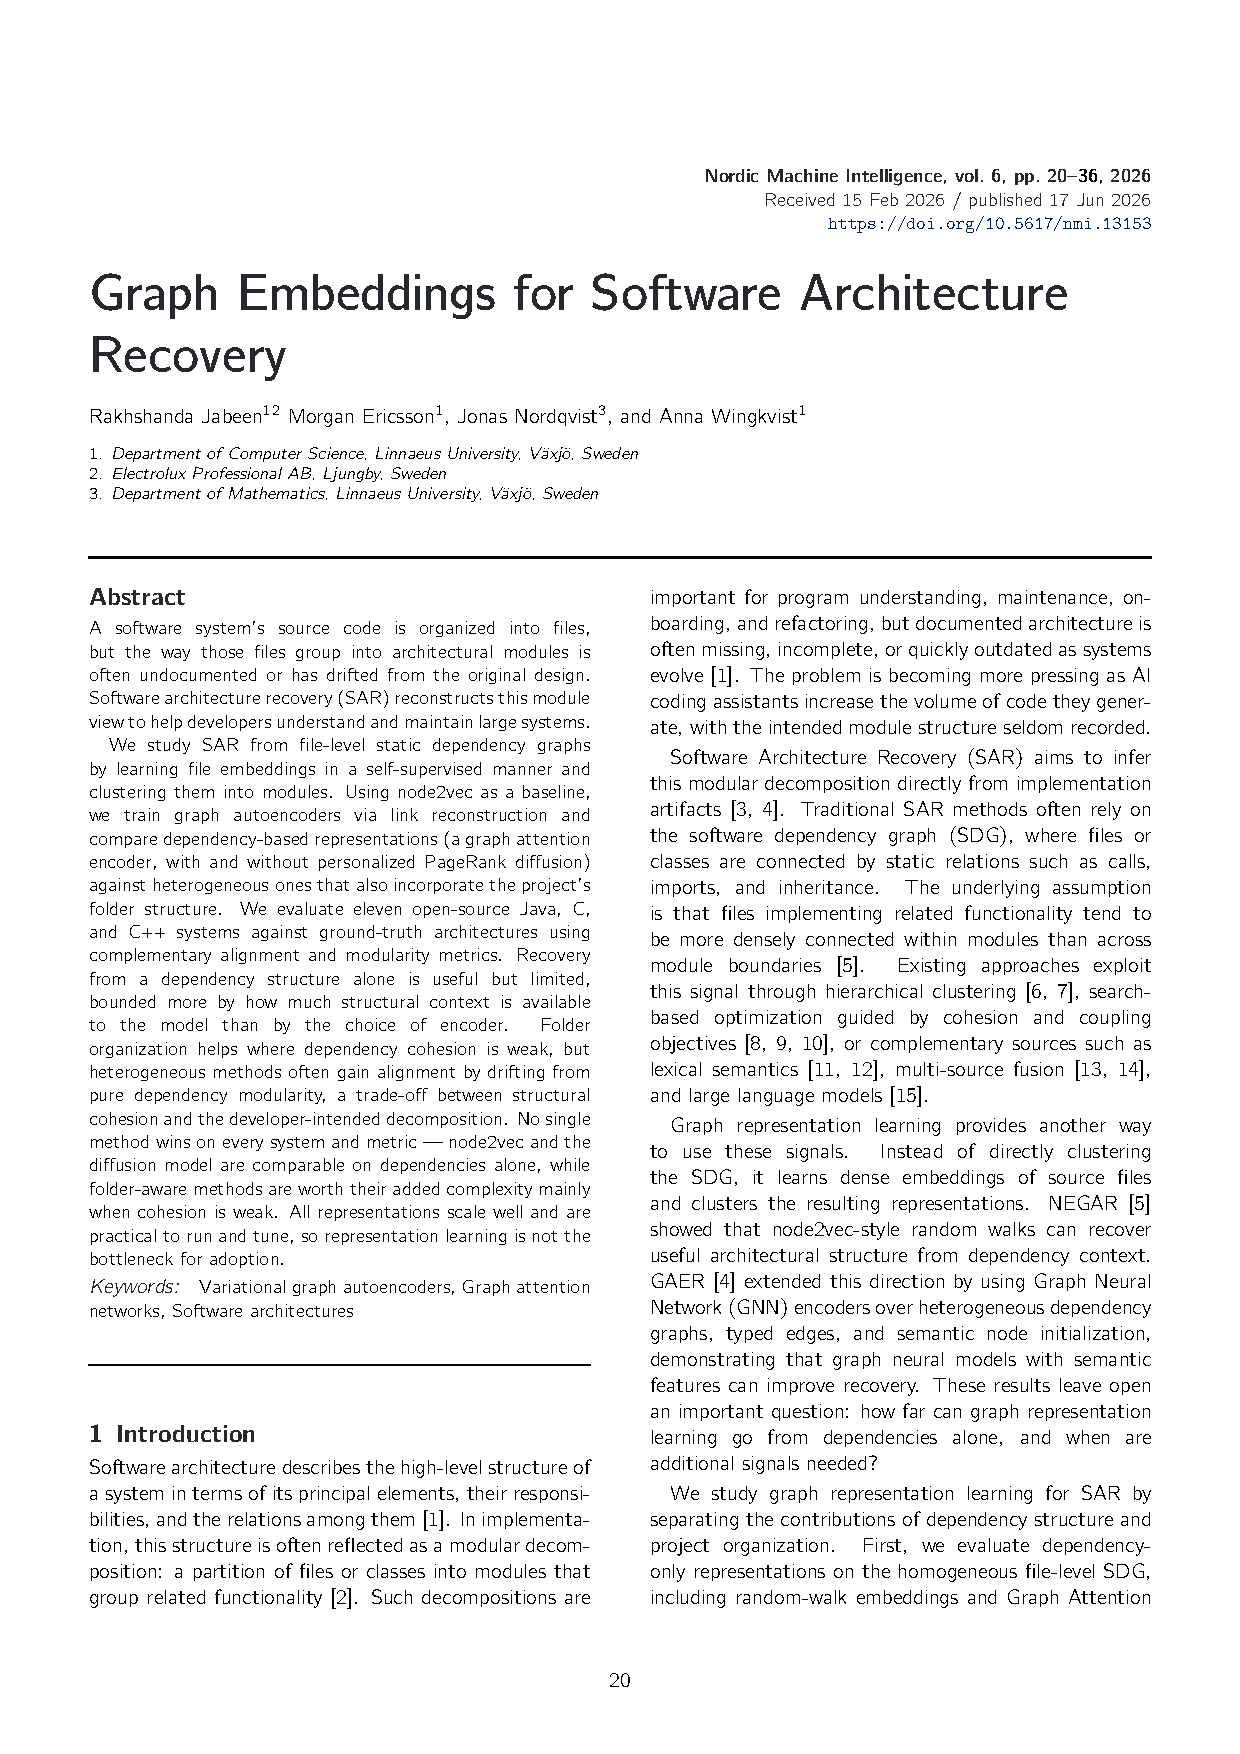
\includepdf[pages=-,pagecommand={}]{papers/StructSAR_1.pdf}
% TODO: addtotoc deferred until page numbers are known from a compiled
% draft.

\renewcommand{\appendixname}{Paper}
\chapter{What Carries Architectural Signal? A Code-to-Architecture Mapping Study}\label{app:publ-hetmap}
\papernumbertab{V}
\myfullciteur{hetmap}
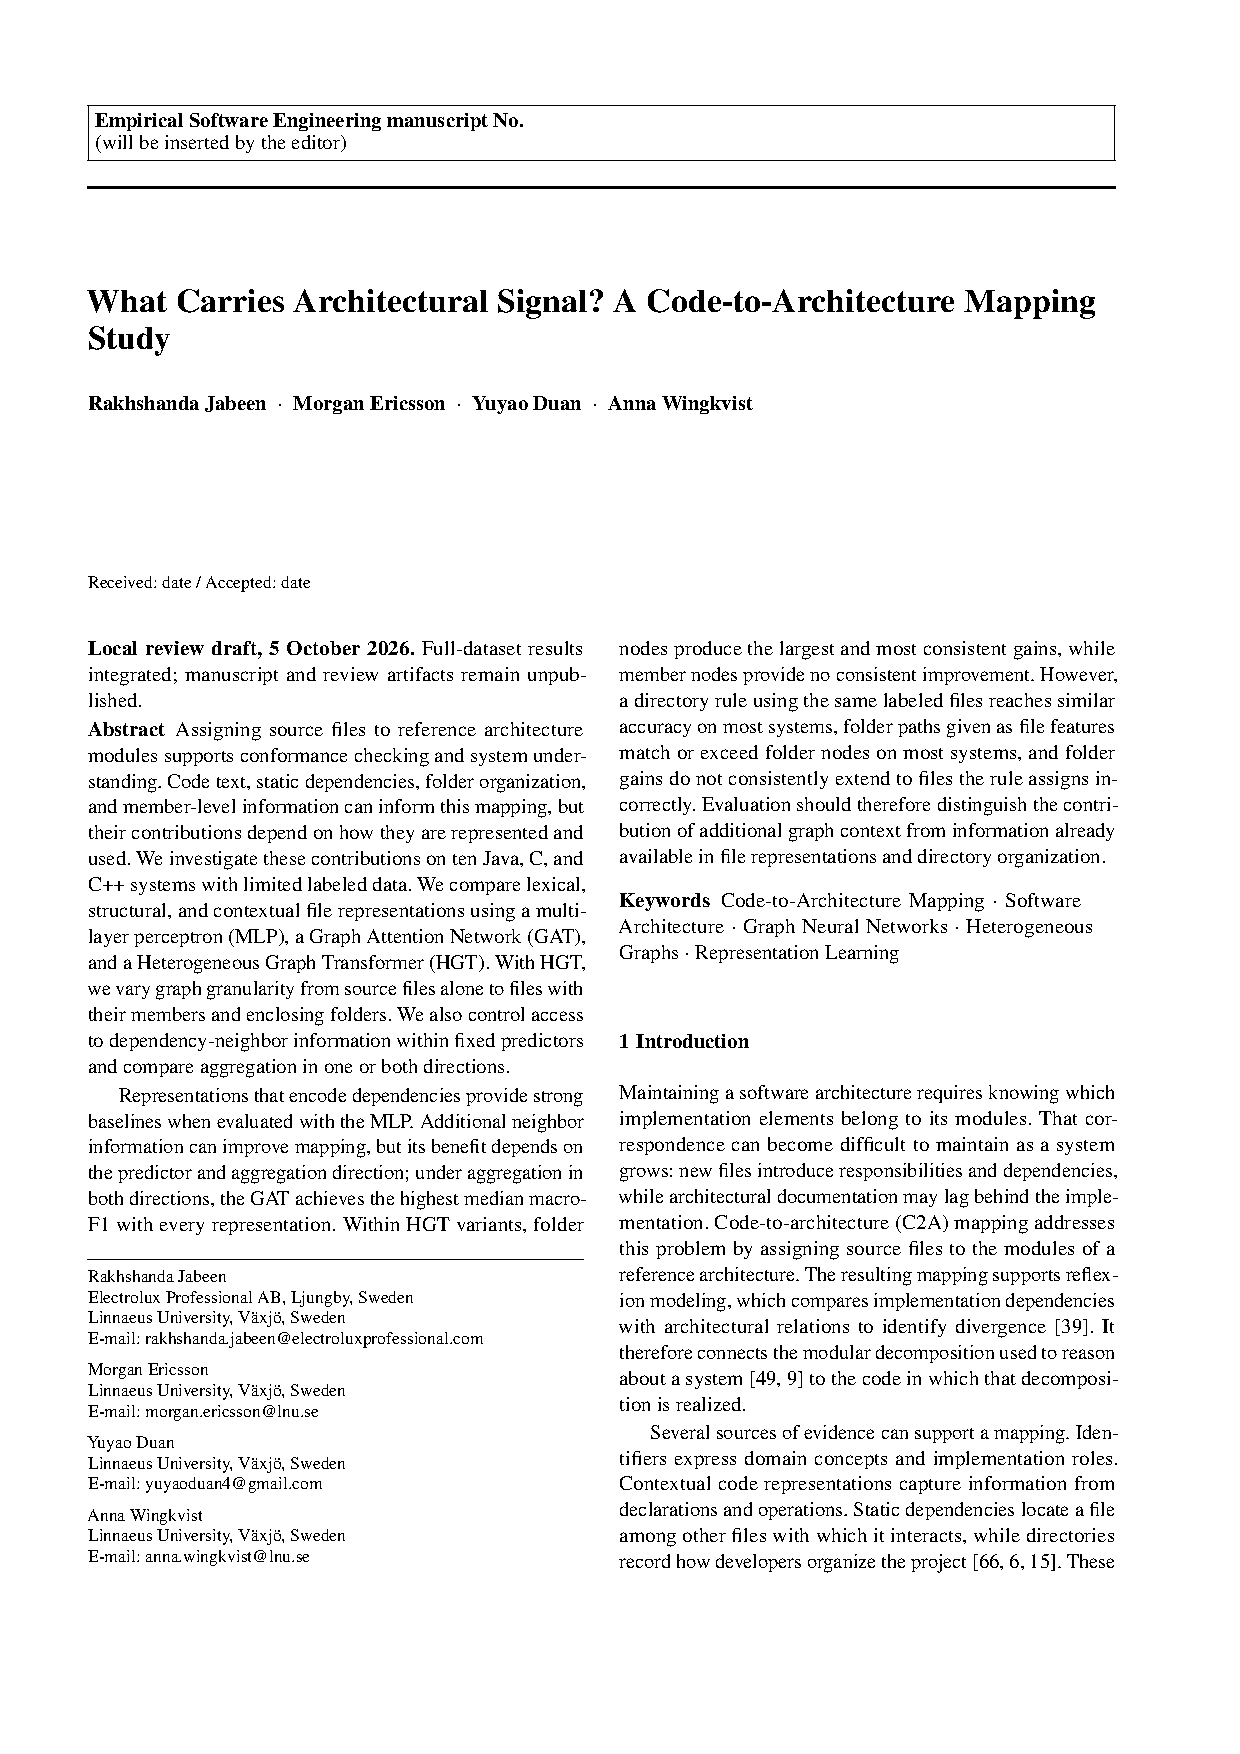
\includepdf[pages=-,pagecommand={}]{papers/HetMap.pdf}
% Manuscript under review (placeholder venue in the .bib entry) -- not
% yet published, so no reuse-rights notice or \includepdf applies.
% Rendered as a citation marked "Under review" until accepted and finalized.

\end{appendices}